\chapter{Introducción específica} % Main chapter title

\label{Chapter2}

%----------------------------------------------------------------------------------------
%	SECTION 1
%----------------------------------------------------------------------------------------
En este capítulo se describen las herramientas, tecnologías y hardware que se utilizó para el desarrollo del sistema.

\section{Protocolos de comunicación}
\label{sec:protocolos}

\subsection{Protocolo HTTP}

HTTP \citep{WEBSITE:HTTP}, por sus siglas en inglés: \textit{Hypertext Transfer Protocol}, es un protocolo de tipo cliente-servidor \citep{WEBSITE:CLIENTESERVIDOR}, mediante el cual se establece una comunicación enviando peticiones y obteniendo respuestas. 

Las características principales de este protocolo son:
\begin{itemize}
	\item Basado en arquitectura cliente-servidor.
	\item Además de hipertexto (HTML \citep{WEBSITE:HTML}) se puede utilizar para transmitir otro tipo de documentos como imágenes o vídeos.
	\item Es un protocolo de capa de aplicación del modelo OSI \citep{WEBSITE:OSI}.
	\item Se transmite principalmente sobre el protocolo TCP\citep{WEBSITE:TCP}.	
\end{itemize}

HTTP define un conjunto de métodos de petición, cada uno indica una acción a ejecutar en el servidor. Los más utilizados son:
\begin{itemize}
	\item GET: se utiliza para recuperar datos.
	\item POST: sirve principalmente para cargar nuevos datos.
	\item PATCH: este método aplica modificaciones parciales a los datos existentes.
	\item PUT: permite reemplazar completamente un registro.
	\item DELETE: elimina datos específicos.	
\end{itemize}


%Si en el texto se hace alusión a diferentes partes del trabajo referirse a ellas como capítulo, sección o subsección según corresponda. Por ejemplo: ``En el capítulo \ref{Chapter1} se explica tal cosa'', o ``En la sección \ref{sec:ejemplo} se presenta lo que sea'', o ``En la subsección \ref{subsec:ejemplo} se discute otra cosa''.
%
%Cuando se quiere poner una lista tabulada, se hace así:
%
%\begin{itemize}
%	\item Este es el primer elemento de la lista.
%	\item Este es el segundo elemento de la lista.
%\end{itemize}
%
%Notar el uso de las mayúsculas y el punto al final de cada elemento.
%
%Si se desea poner una lista numerada el formato es este:
%
%\begin{enumerate}
%	\item Este es el primer elemento de la lista.
%	\item Este es el segundo elemento de la lista.
%\end{enumerate}
%
%Notar el uso de las mayúsculas y el punto al final de cada elemento.

\subsection{Protocolo MQTT}
\label{subsec:mqtt}

MQTT \citep{WEBSITE:MQTT} son las siglas de \textit{Message Queuing Telemetry Transport}. Se trata de un protocolo de mensajería liviano para usar en casos donde existen recursos limitados de ancho de banda. 

Se transmite sobre protocolo TCP en la arquitectura publish/subscribe \citep{WEBSITE:PUBSUB}.

Los roles que intervienen en un protocolo MQTT son los siguientes:
\begin{itemize}
	\item Publicadores: son los que envían los datos.
	\item Suscriptores: son los que consumen los datos.
	\item Broker: Transmite los mensajes publicados a los suscriptores.	
\end{itemize}

Un cliente puede ser publicador, suscriptor o ambos. El broker es el punto central de la comunicación ya que sin este los mensajes nunca llegarían a destino. 

En la figura \ref{fig:mqttArq} se puede apreciar un ejemplo de comunicación en la arquitectura MQTT.


\begin{figure}[ht]
	\centering
	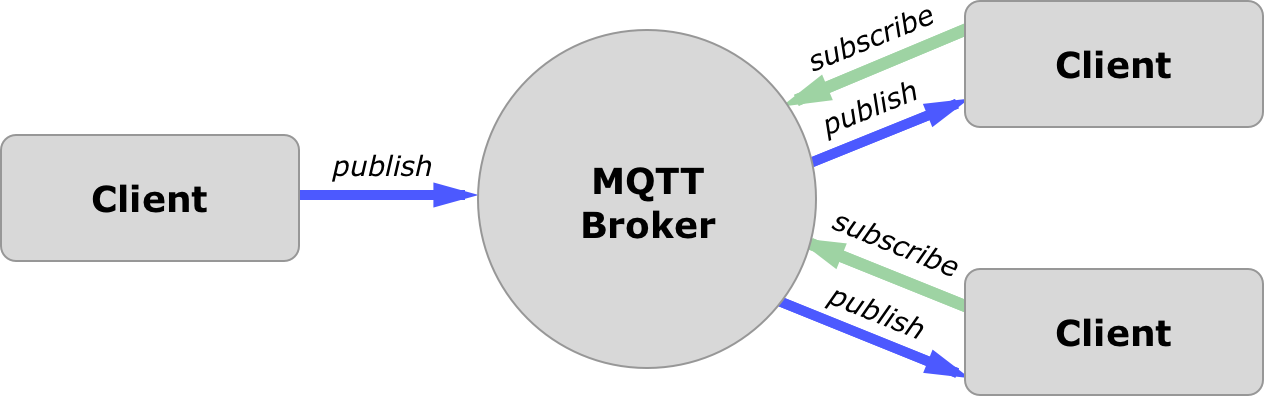
\includegraphics[scale=.25]{./Figures/mqtt-diagram.png}
	\caption{Arquitectura MQTT publish/subscribe.}
	\label{fig:mqttArq}
\end{figure}

La estructura de mensajes en este protocolo se dividen en dos: \textit{topics} los cuales son de tipo jerárquicos, utilizando la barra (/) como separador, y \textit{payload} en dónde se incluye el mensaje que se quiere transmitir. Por ejemplo: topic: "nodos/procesos/guardar", payload:"mensaje de ejemplo". Siguiendo este ejemplo un cliente podría suscribirse a ese topic o a una jerarquía más alta y recibir todos los mensajes de los topics que comiencen con nodo/procesos. 

\subsection{Ecliplse Mosquitto}
\label{subsec:mosquitto}

Eclipse Mosquitto \citep{WEBSITE:MOSQUITTO} es un broker MQTT OpenSource liviano y adecuado para utilizar en todo tipo de dispositivos sobre todo aquellos que cuenten con baja potencia como microcontroladores.

El objetivo de Mosquitto es proporcionar una implementación ligera y de bajo consumo de recursos para permitir la comunicación entre dispositivos IoT en redes con ancho de banda limitado y recursos de memoria.

Mosquitto es compatible con una amplia gama de lenguajes de programación, lo que lo hace fácilmente integrable con diferentes aplicaciones. Además, cuenta con una arquitectura flexible y escalable que permite su implementación en dispositivos con diferentes capacidades de procesamiento y memoria.

Otra característica importante de este broker es su capacidad para manejar conexiones seguras a través del uso de protocolos de seguridad como SSL/TLS y SASL. Esto permite la comunicación segura y cifrada entre dispositivos de IoT en diferentes entornos de red.	

\section{Bases de datos}
\label{sec:ddbb}

Las bases de datos son una parte esencial de cualquier aplicación IoT, ya que se utilizan para almacenar y gestionar los datos recopilados por los dispositivos IoT. En esta sección, se describen las tecnologías utilizadas en bases de datos.

\subsection{Bases de datos relacionales}
\label{subsec:RDBMS}

Las bases de datos relacionales son un tipo de sistema de gestión de bases de datos (SGBD) que se basa en el modelo de datos relacional. Este modelo se utiliza para organizar y almacenar datos en tablas, donde cada tabla representa una entidad o concepto del mundo real y cada fila representa una instancia de esa entidad.

Las tablas se relacionan entre sí mediante claves primarias y claves externas, lo que permite establecer relaciones entre las entidades y realizar consultas complejas que combinan datos de varias tablas. Además, las bases de datos relacionales utilizan el lenguaje de consulta estructurado (SQL o \textit{Structured Query Language}) para interactuar con los datos almacenados en la base de datos.

En la figura \ref{fig:relddbb} se puede apreciar un ejemplo de un diagrama de base de datos relacional con sus tablas, filas y relaciones.

\begin{figure}[ht]
	\centering
	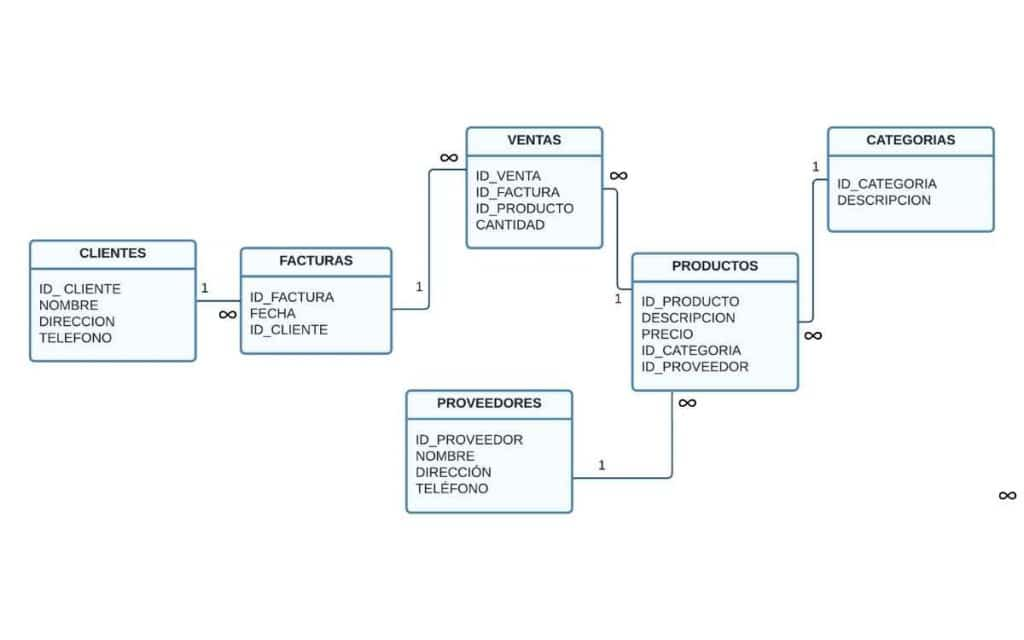
\includegraphics[scale=.40]{./Figures/relddbb.jpg}
	\caption{Diagrama base de datos relacional.}
	\label{fig:relddbb}
\end{figure}

\subsection{MySql}
\label{subsec:mysql}

MySql \citep{WEBSITE:mysql-site} es un sistema de gestión de bases de datos relacional y de código abierto, que utiliza el lenguaje SQL para interactuar con los datos almacenados en la base de datos. 

Ofrece una amplia gama de características avanzadas, como soporte para transacciones ACID, índices avanzados, clústeres de alta disponibilidad y replicación. Además, admite múltiples lenguajes de programación, incluyendo C, C++, Python, Java y Ruby, lo que lo hace extremadamente flexible y escalable.

Tiene múltiples capas de seguridad integradas en el sistema, incluyendo autenticación y control de acceso basado en roles. 

Debido a su combinación de características avanzadas, flexibilidad y seguridad, MySql se utiliza ampliamente en aplicaciones de misión crítica y de alta disponibilidad, incluyendo aplicaciones IoT.

\section{Tecnologías backend}
\label{sec:backend}

Las tecnologías backend se utilizan para desarrollar la lógica de la aplicación y gestionar la comunicación entre el servidor y los dispositivos IoT. En esta sección, se describen las tecnologías backend utilizadas.

\subsection{API RESTFul}
\label{subsec:apis}

Las APIs RESTful \textit{(Representational State Transfer)} son una arquitectura de diseño de aplicaciones web que utiliza el protocolo HTTP para transferir datos. Las API RESTful están diseñadas para ser escalables, flexibles y fáciles de entender para los desarrolladores y los clientes que las consumen.

Están basadas en el concepto de recursos, que son objetos o conjuntos de datos que se pueden acceder a través de una URI (Identificador de recurso uniforme, por sus siglas en inglés). Cada recurso tiene un conjunto de operaciones que se pueden realizar sobre él, como GET (para obtener los datos del recurso), POST (para crear un nuevo recurso), PUT (para actualizar un recurso existente) y DELETE (para eliminar un recurso).

En la figura \ref{fig:apirest} se puede apreciar un ejemplo de una arquitectura API rest, incluyendo la petición o \textit{request} del usuario en formato JSON, el método HTTP y la respuesta o \textit{response} del servidor.

\begin{figure}[ht]
	\centering
	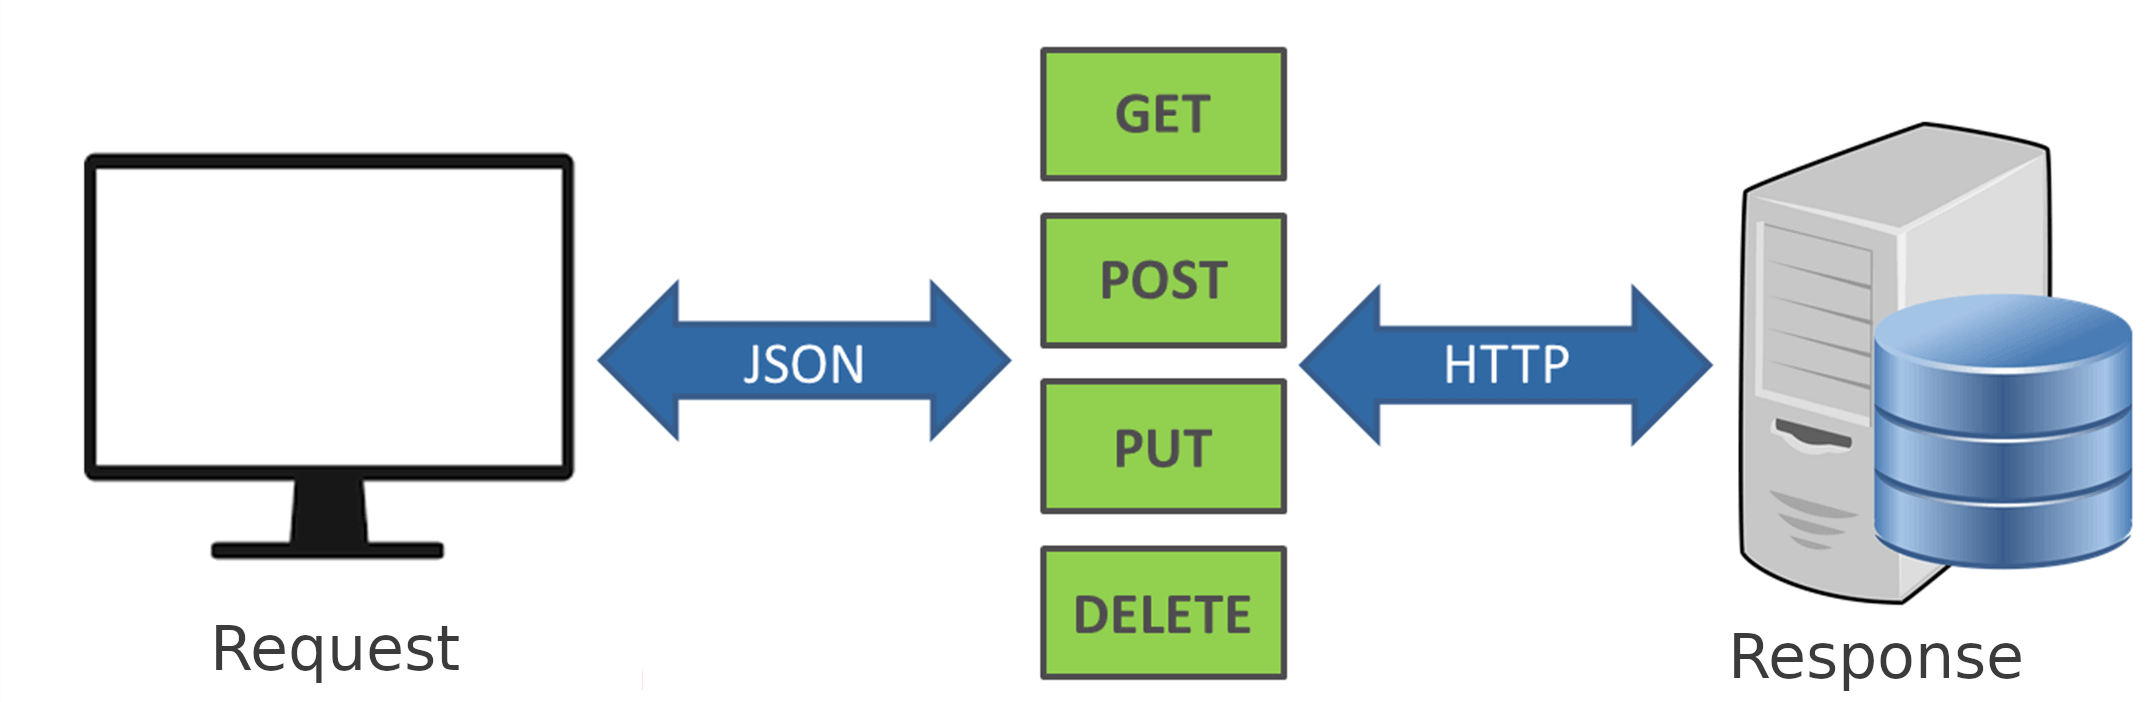
\includegraphics[scale=.15]{./Figures/apirest.png}
	\caption{Arquitectura API Rest.}
	\label{fig:apirest}
\end{figure}

\subsection{Node.js}
\label{subsec:nodejs}

Node.js es un entorno de tiempo de ejecución de JavaScript de código abierto que se ejecuta en el servidor. Fue creado en 2009 con el objetivo de poder desarrollar aplicaciones escalables y de alto rendimiento utilizando el mismo lenguaje de programación para el lado del servidor y del cliente.

Se basa en el motor de JavaScript V8 de Google, lo que lo hace muy rápido y eficiente. Utiliza un modelo de E/S sin bloqueo y orientado a eventos, lo que significa que es capaz de manejar un gran número de solicitudes simultáneas sin bloquear el proceso. Esto lo hace especialmente adecuado para aplicaciones web en tiempo real y aplicaciones de transmisión de medios.

También cuenta con una amplia variedad de módulos y bibliotecas disponibles a través de su gestor de paquetes NPM. Esto permite aprovechar funcionalidades existentes, desde la creación de APIs RESTful hasta la manipulación de archivos, la comunicación con dispositivos y bases de datos.

\subsection{Express}
\label{subsec:express}

Express es un popular framework de Node.js utilizado para la creación de aplicaciones web y APIs RESTful. Fue creado en 2010 y es mantenido por la comunidad de desarrolladores de Node.js.

Proporciona una serie de funcionalidades para simplificar el proceso de creación de aplicaciones web. Entre ellas se incluyen el manejo de rutas, la gestión de middleware, la manipulación de sesiones y cookies, la autenticación de usuarios y la integración con bases de datos.

En Express, el manejo de rutas se realiza mediante la definición de las rutas y los controladores correspondientes. Las rutas son los patrones utilizados para identificar las solicitudes HTTP entrantes que serán atendidas por la aplicación web. Los controladores son las funciones que se encargan de procesar esas solicitudes y generar la respuesta adecuada.

Para definir una ruta, se utiliza el método correspondiente al verbo HTTP que se desea manejar (GET, POST, PUT, DELETE, etc.), seguido de la ruta o patrón que se desea asociar a esa solicitud. 

\subsection{Sequelize}
\label{subsec:sequelize}

Sequelize es una librería de ORM \textit{(Object-Relational Mapping)} para Node.js que permite trabajar con bases de datos relacionales como MySQL, PostgreSQL, SQLite, y MSSQL. Facilita el acceso a la base de datos y permite la creación de consultas a través de una interfaz de programación de aplicaciones (API) de alto nivel basada en objetos.

Se utiliza junto a Express y Node.js para simplificar el proceso de acceso y manipulación de datos en bases de datos relacionales. Al utilizar Sequelize, se pueden crear modelos de datos que representen las tablas de la base de datos, lo que permite interactuar con la base de datos utilizando objetos en lugar de consultas SQL.

\section{Tecnologías frontend}
\label{sec:frontend}

Las tecnologías frontend son aquellas que se utilizan para crear la parte visual y de interacción de una aplicación web o móvil. Estas tecnologías se enfocan en la presentación y manipulación de la interfaz de usuario, en la interacción con el usuario final y actúa como intermediario entre el usuario final y el backend de la aplicación.

Algunas de las tecnologías frontend más comunes son:
\begin{itemize}
	\item HTML \textit{(HyperText Markup Language)}: Es el lenguaje de marcado que se utiliza para estructurar y dar formato al contenido de una página web.
	\item CSS \textit{(Cascading Style Sheets)}: Es el lenguaje utilizado para dar estilo y diseño a una página web, permitiendo la personalización de fuentes, colores, márgenes, tamaños y otros aspectos visuales.
	\item JavaScript: Es un lenguaje de programación que se utiliza para hacer que la página web sea interactiva y dinámica, permitiendo la manipulación de elementos del DOM, eventos, animaciones y otras acciones en el lado del cliente.
	\item Frameworks de JavaScript: Son librerías que permiten simplificar el desarrollo de aplicaciones web, proporcionando funcionalidades predefinidas y estructuras de organización.
	\item Bibliotecas de diseño: Son herramientas que ofrecen componentes visuales predefinidos y estilos de diseño que permiten crear páginas web con un aspecto más profesional y elegante.
	\item Herramientas de gestión de paquetes: Son programas que permiten gestionar las dependencias de los proyectos y mantener actualizadas las librerías utilizadas en el desarrollo.	
\end{itemize}

\subsection{Ionic framework}
\label{subsec:ionic}

Ionic es un framework de desarrollo de aplicaciones móviles híbridas basado en tecnologías web como HTML, CSS y JavaScript. Permite crear aplicaciones móviles para iOS, Android y la web utilizando un conjunto de herramientas y librerías predefinidas.

Ofrece una gran cantidad de componentes visuales, animaciones y funcionalidades para crear aplicaciones móviles con una apariencia y experiencia de usuario nativa, similar a las aplicaciones desarrolladas con tecnologías nativas como Java para Android o Swift para iOS. Además, permite la integración con otras tecnologías como Angular y React.

El uso de tecnologías web permite el desarrollo de aplicaciones móviles de forma más rápida y sencilla que las aplicaciones nativas, ya que se utiliza un único código base que se puede adaptar para cada plataforma. Además, ofrece una gran cantidad de herramientas y servicios para simplificar el proceso de desarrollo, como Ionic Native (para el acceso a las características nativas del dispositivo) y Ionic Appflow (para la implementación continua y la gestión de versiones).

%En resumen, Ionic es una herramienta muy útil para el desarrollo de aplicaciones móviles híbridas utilizando tecnologías web, que permite crear aplicaciones con una apariencia y experiencia de usuario nativa, y que simplifica el proceso de desarrollo gracias a su conjunto de herramientas y servicios predefinidos.

\section{Tecnologías de servidor}
\label{sec:servidor}

\subsection{Docker y Docker Compose}
\label{subsec:docker}

Docker es una plataforma de software libre que se utiliza para desarrollar, implementar y ejecutar aplicaciones en contenedores. Los contenedores son una forma de virtualización que permiten a los desarrolladores empaquetar una aplicación y todas sus dependencias en una imagen de contenedor, que se puede ejecutar en cualquier entorno que tenga Docker instalado. Docker facilita la implementación de aplicaciones en diferentes plataformas, desde servidores locales hasta nubes públicas.

Docker Compose es una herramienta de Docker que se utiliza para definir y ejecutar aplicaciones de múltiples contenedores. Permite definir todos los servicios necesarios para una aplicación en un archivo de configuración YAML, lo que facilita la implementación y el mantenimiento de la aplicación. Docker Compose puede iniciar todos los contenedores necesarios para la aplicación con un solo comando, lo que ahorra tiempo y reduce los errores.

\subsection{Servidor web Nginx}
\label{subsec:servidorweb}

Un servidor web es un software que procesa solicitudes HTTP de clientes y responde con contenido estático o dinámico. Los servidores web se utilizan para alojar y servir sitios web y aplicaciones web. Un servidor web típicamente aloja varios sitios web y puede gestionar múltiples solicitudes HTTP simultáneamente.

Nginx es un servidor web de código abierto que se utiliza para alojar y servir sitios web y aplicaciones web. Nginx es conocido por su alta escalabilidad, rendimiento y capacidad de manejar múltiples solicitudes HTTP simultáneamente. Es un servidor web ligero y rápido que se puede utilizar como un proxy inverso para distribuir la carga de trabajo a diferentes servidores y balancear la carga de tráfico.

%Se recomienda no utilizar \textbf{texto en negritas} en ningún párrafo, ni tampoco texto \underline{subrayado}. En cambio sí se debe utilizar \textit{texto en itálicas} para palabras en un idioma extranjero, al menos la primera vez que aparecen en el texto. En el caso de palabras que estamos inventando se deben utilizar ``comillas'', así como también para citas textuales. Por ejemplo, un \textit{digital filter} es una especie de ``selector'' que permite separar ciertos componentes armónicos en particular.
%
%La escritura debe ser impersonal. Por ejemplo, no utilizar ``el diseño del firmware lo hice de acuerdo con tal principio'', sino ``el firmware fue diseñado utilizando tal principio''. 
%
%El trabajo es algo que al momento de escribir la memoria se supone que ya está concluido, entonces todo lo que se refiera a hacer el trabajo se narra en tiempo pasado, porque es algo que ya ocurrió. Por ejemplo, "se diseñó el firmware empleando la técnica de test driven development".
%
%En cambio, la memoria es algo que está vivo cada vez que el lector la lee. Por eso transcurre siempre en tiempo presente, como por ejemplo:
%
%``En el presente capítulo se da una visión global sobre las distintas pruebas realizadas y los resultados obtenidos. Se explica el modo en que fueron llevados a cabo los test unitarios y las pruebas del sistema''.
%
%Se recomienda no utilizar una sección de glosario sino colocar la descripción de las abreviaturas como parte del mismo cuerpo del texto. Por ejemplo, RTOS (\textit{Real Time Operating System}, Sistema Operativo de Tiempo Real) o en caso de considerarlo apropiado mediante notas a pie de página.
%
%Si se desea indicar alguna página web utilizar el siguiente formato de referencias bibliográficas, dónde las referencias se detallan en la sección de bibliografía de la memoria, utilizado el formato establecido por IEEE en \citep{IEEE:citation}. Por ejemplo, ``el presente trabajo se basa en la plataforma EDU-CIAA-NXP \citep{CIAA}, la cual...''.
%
%\subsection{Figuras} 
%
%Al insertar figuras en la memoria se deben considerar determinadas pautas. Para empezar, usar siempre tipografía claramente legible. Luego, tener claro que \textbf{es incorrecto} escribir por ejemplo esto: ``El diseño elegido es un cuadrado, como se ve en la siguiente figura:''
%
%\begin{figure}[h]
%\centering
%\includegraphics[scale=.45]{./Figures/cuadradoAzul.png}
%\end{figure}
%
%La forma correcta de utilizar una figura es con referencias cruzadas, por ejemplo: ``Se eligió utilizar un cuadrado azul para el logo, como puede observarse en la figura \ref{fig:cuadradoAzul}''.
%
%\begin{figure}[ht]
%	\centering
%	\includegraphics[scale=.45]{./Figures/cuadradoAzul.png}
%	\caption{Ilustración del cuadrado azul que se eligió para el diseño del logo.\protect\footnotemark.}
%	\label{fig:cuadradoAzul}
%\end{figure}
%
%\footnotetext{Imagen tomada de \url{https://goo.gl/images/i7C70w}}
%
%
%El texto de las figuras debe estar siempre en español, excepto que se decida reproducir una figura original tomada de alguna referencia. En ese caso la referencia de la cual se tomó la figura debe ser indicada en el epígrafe de la figura e incluida como una nota al pie, como se ilustra en la figura \ref{fig:palabraIngles}.
%
%\begin{figure}[htpb]
%	\centering
%	\includegraphics[scale=.3]{./Figures/word.jpeg}
%	\caption{Imagen tomada de la página oficial del procesador\protect\footnotemark.}
%	\label{fig:palabraIngles}
%\end{figure}
%
%\footnotetext{Imagen tomada de \url{https://goo.gl/images/i7C70w}}
%
%La figura y el epígrafe deben conformar una unidad cuyo significado principal pueda ser comprendido por el lector sin necesidad de leer el cuerpo central de la memoria. Para eso es necesario que el epígrafe sea todo lo detallado que corresponda y si en la figura se utilizan abreviaturas entonces aclarar su significado en el epígrafe o en la misma figura.
%
%
%
%\begin{figure}[ht]
%	\centering
%	\includegraphics[scale=.37]{./Figures/questionMark.png}
%	\caption{¿Por qué de pronto aparece esta figura?}
%	\label{fig:questionMark}
%\end{figure}
%
%Nunca colocar una figura en el documento antes de hacer la primera referencia a ella, como se ilustra con la figura \ref{fig:questionMark}, porque sino el lector no comprenderá por qué de pronto aparece la figura en el documento, lo que distraerá su atención.
%
%Otra posibilidad es utilizar el entorno \textit{subfigure} para incluir más de una figura, como se puede ver en la figura \ref{fig:three graphs}. Notar que se pueden referenciar también las figuras internas individualmente de esta manera: \ref{fig:1de3}, \ref{fig:2de3} y \ref{fig:3de3}.
% 
%\begin{figure}[!htpb]
%     \centering
%     \begin{subfigure}[b]{0.3\textwidth}
%         \centering
%         \includegraphics[width=.65\textwidth]{./Figures/questionMark}
%         \caption{Un caption.}
%         \label{fig:1de3}
%     \end{subfigure}
%     \hfill
%     \begin{subfigure}[b]{0.3\textwidth}
%         \centering
%         \includegraphics[width=.65\textwidth]{./Figures/questionMark}
%         \caption{Otro.}
%         \label{fig:2de3}
%     \end{subfigure}
%     \hfill
%     \begin{subfigure}[b]{0.3\textwidth}
%         \centering
%         \includegraphics[width=.65\textwidth]{./Figures/questionMark}
%         \caption{Y otro más.}
%         \label{fig:3de3}
%     \end{subfigure}
%        \caption{Tres gráficos simples}
%        \label{fig:three graphs}
%\end{figure}
%
%El código para generar las imágenes se encuentra disponible para su reutilización en el archivo \file{Chapter2.tex}.
%
%\subsection{Tablas}
%
%Para las tablas utilizar el mismo formato que para las figuras, sólo que el epígrafe se debe colocar arriba de la tabla, como se ilustra en la tabla \ref{tab:peces}. Observar que sólo algunas filas van con líneas visibles y notar el uso de las negritas para los encabezados.  La referencia se logra utilizando el comando \verb|\ref{<label>}| donde label debe estar definida dentro del entorno de la tabla.
%
%\begin{verbatim}
%\begin{table}[h]
%	\centering
%	\caption[caption corto]{caption largo más descriptivo}
%	\begin{tabular}{l c c}    
%		\toprule
%		\textbf{Especie}     & \textbf{Tamaño} & \textbf{Valor}\\
%		\midrule
%		Amphiprion Ocellaris & 10 cm           & \$ 6.000 \\		
%		Hepatus Blue Tang    & 15 cm           & \$ 7.000 \\
%		Zebrasoma Xanthurus  & 12 cm           & \$ 6.800 \\
%		\bottomrule
%		\hline
%	\end{tabular}
%	\label{tab:peces}
%\end{table}
%\end{verbatim}
%
%
%\begin{table}[h]
%	\centering
%	\caption[caption corto]{caption largo más descriptivo}
%	\begin{tabular}{l c c}    
%		\toprule
%		\textbf{Especie} 	 & \textbf{Tamaño} 		& \textbf{Valor}  \\
%		\midrule
%		Amphiprion Ocellaris & 10 cm 				& \$ 6.000 \\		
%		Hepatus Blue Tang	 & 15 cm				& \$ 7.000 \\
%		Zebrasoma Xanthurus	 & 12 cm				& \$ 6.800 \\
%		\bottomrule
%		\hline
%	\end{tabular}
%	\label{tab:peces}
%\end{table}
%
%En cada capítulo se debe reiniciar el número de conteo de las figuras y las tablas, por ejemplo, figura 2.1 o tabla 2.1, pero no se debe reiniciar el conteo en cada sección. Por suerte la plantilla se encarga de esto por nosotros.
%
%\subsection{Ecuaciones}
%\label{sec:Ecuaciones}
%
%Al insertar ecuaciones en la memoria dentro de un entorno \textit{equation}, éstas se numeran en forma automática  y se pueden referir al igual que como se hace con las figuras y tablas, por ejemplo ver la ecuación \ref{eq:metric}.
%
%\begin{equation}
%	\label{eq:metric}
%	ds^2 = c^2 dt^2 \left( \frac{d\sigma^2}{1-k\sigma^2} + \sigma^2\left[ d\theta^2 + \sin^2\theta d\phi^2 \right] \right)
%\end{equation}
%                                                        
%Es importante tener presente que si bien las ecuaciones pueden ser referidas por su número, también es correcto utilizar los dos puntos, como por ejemplo ``la expresión matemática que describe este comportamiento es la siguiente:''
%
%\begin{equation}
%	\label{eq:schrodinger}
%	\frac{\hbar^2}{2m}\nabla^2\Psi + V(\mathbf{r})\Psi = -i\hbar \frac{\partial\Psi}{\partial t}
%\end{equation}
%
%Para generar la ecuación \ref{eq:metric} se utilizó el siguiente código:
%
%\begin{verbatim}
%\begin{equation}
%	\label{eq:metric}
%	ds^2 = c^2 dt^2 \left( \frac{d\sigma^2}{1-k\sigma^2} + 
%	\sigma^2\left[ d\theta^2 + 
%	\sin^2\theta d\phi^2 \right] \right)
%\end{equation}
%\end{verbatim}
%
%Y para la ecuación \ref{eq:schrodinger}:
%
%\begin{verbatim}
%\begin{equation}
%	\label{eq:schrodinger}
%	\frac{\hbar^2}{2m}\nabla^2\Psi + V(\mathbf{r})\Psi = 
%	-i\hbar \frac{\partial\Psi}{\partial t}
%\end{equation}
%
%\end{verbatim}